\documentclass[paper=a4, fontsize=11pt]{scrartcl} % A4 paper and 11pt font size

\usepackage[T1]{fontenc} % Use 8-bit encoding that has 256 glyphs
\usepackage[english]{babel} % English language/hyphenation
\usepackage{amsmath,amsfonts,amsthm} % Math packages
\usepackage{graphicx}
\usepackage{sectsty} % Allows customizing section commands
\allsectionsfont{ \normalfont\scshape} % Make all sections centered, the default font and small caps

\usepackage{fancyhdr} % Custom headers and footers
\pagestyle{fancyplain} % Makes all pages in the document conform to the custom headers and footers
\fancyhead{} % No page header - if you want one, create it in the same way as the footers below
\fancyfoot[L]{} % Empty left footer
\fancyfoot[C]{} % Empty center footer
\fancyfoot[R]{\thepage} % Page numbering for right footer
\renewcommand{\headrulewidth}{0pt} % Remove header underlines
\renewcommand{\footrulewidth}{0pt} % Remove footer underlines
\setlength{\headheight}{13.6pt} % Customize the height of the header


%----------------------------------------------------------------------------------------
%	TITLE SECTION
%----------------------------------------------------------------------------------------

\newcommand{\horrule}[1]{\rule{\linewidth}{#1}} % Create horizontal rule command with 1 argument of height

\title{	
\normalfont \normalsize 
\textsc{Indian Institute of Technology Delhi} \\ [25pt] % Your university, school and/or department name(s)
\horrule{0.5pt} \\[0.4cm] % Thin top horizontal rule
\huge Lamp Post Measurement \\ % The assignment title
\horrule{2pt} \\[0.5cm] % Thick bottom horizontal rule
}

\author{Suyash Agrawal \\ 2015CS10262} % Your name

\date{\normalsize\today} % Today's date or a custom date

\begin{document}

\maketitle % Print the title

\section{Measuring Height}

\subsection{Assumptions}
\begin{itemize}
\item We require the field of view of the camera. Either this can be given in specifications itself or this can be easily calculated by placing an object of known length at a known distance from camera (this gives us the angle subtended ) and dividing the angle with the ratio of the length of object in image by image height. Let us denote the field of view of camera by $\Omega$.
\item We assume the camera to be kept on the ground and thus field of vision will be reduced by half.
\item The object is sufficiently far away that whole of it is visible in the image.
\end{itemize}

\subsection{Basic Equations}

\begin{figure}[ht!]
		\centering
		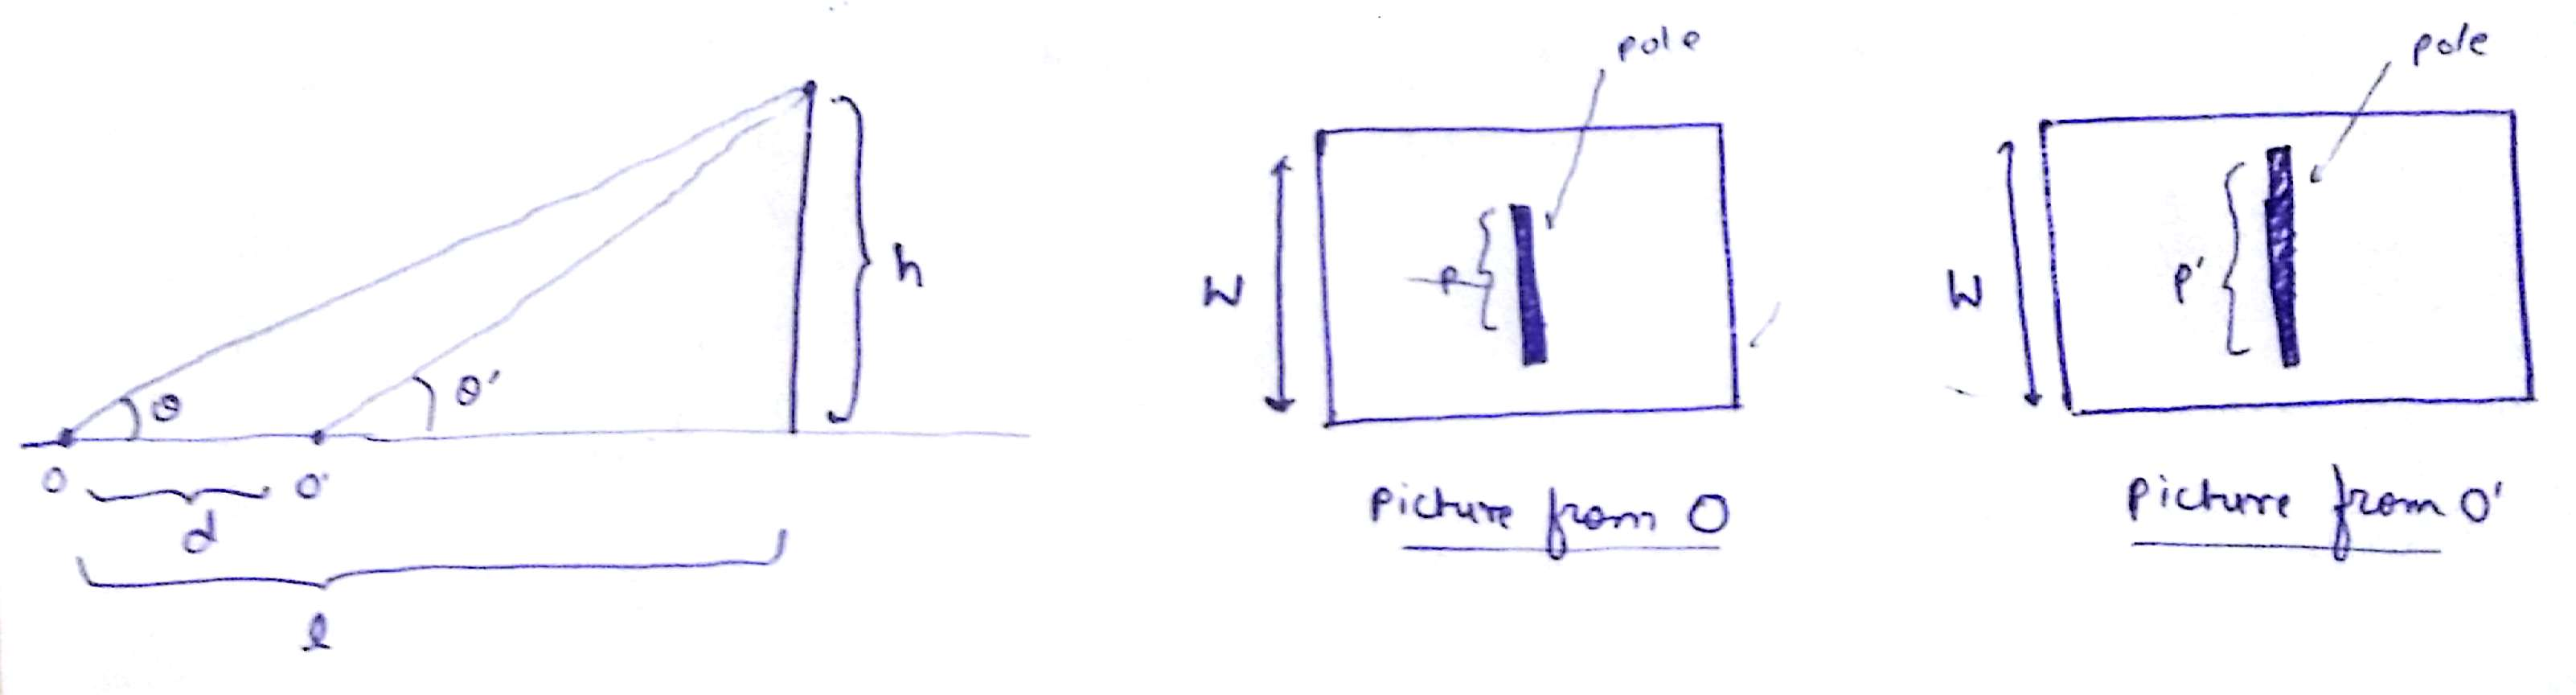
\includegraphics[width=0.8\textwidth]{diagram.jpg}
		\caption{Diagram of situation}
		\centering
\end{figure}


\begin{equation} \label{eq1}
  \tan\theta = \frac{h}{l}
\end{equation}

\begin{equation} \label{eq2}
  \tan\theta' = \frac{h}{l-d}
\end{equation}

\begin{equation} \label{eq3}
  \frac{p'}{p} = \frac{\theta'}{\theta}
\end{equation}

\begin{equation} \label{eq4}
  \frac{p}{W} = \frac{theta}{\Omega/2}
\end{equation}

From equation \ref{eq1} and equation \ref{eq2}:
\begin{equation} \label{eq5}
  h = \frac{d\tan\theta\tan\theta'}{\tan\theta' - \tan\theta}
\end{equation}



\subsection{Procedure}

\begin{enumerate}
\item Take a picture from unknown distance $l$ of the pole. Let the real height of pole be $h$ (vertically from ground). Let picture height be $w$ and height of pole in picture be $p$.
\item Move $d$ distance towards the pole and take a picture. Let the new height of pole in picture be $p'$ .
\item Now using equation \ref{eq4} we can measure angle $\theta$ and using equation \ref{eq3} we can measure angle $\theta'$ .
\item Then using equation \ref{eq5} we measure the vertical height $h$ of pole from ground. 
\end{enumerate}

\section{Measuring Inclination}
\begin{enumerate}
\item First measure the actual length of pole using:\\
\begin{equation}
  L = (\text{Length of inclined post in pixel}) * \frac{h}{p}.
\end{equation}
\item Then calculate the inclination from vertical using : $\theta_a$ = $\cos^{-1}(L/h)$ 
\end{enumerate}

\end{document}